\section{Implementation and Evaluation} \label{Evaluation}

\subsection{Implementation}

We implement a prototype of \textit{ScalIMS} in Java and deploy \textit{ScalIMS} code on both local controller and global controller. The local controller is implemented as a module in the FloodLight SDN controller~\cite{floodlight}. The global controller is implemented as a multi-threaded server program, which communicates with local controllers over regular sockets.  We also implement a traffic generator based on PJSIP~\cite{pjsip}. We deploy one traffic generator in each datacenter, producing user arrivals bound to the datacenter at a configurable rate. A global traffic generator coordinator receives notifications of generated users and pairs up users in a first-come-first-match manner. A call process is launched between every pair of paired users, which includes SIP transactions to establish a call, followed by a one-minute voice call at the bit rate of 80kbit/s, as well as necessary SIP transactions to shutdown the call.

%We use the P-CSCF, S-CSCF and HSS components from Project Clearwater as our control plane network functions. For data plane network functions, we use a firewall (implemented using user space click), a intrusion detector (Snort) and a transcoder (implemented using user space click). Each network function runs in QEMU/KVM virtual machine. The virtual machine has a uniform configuration of 2 cores and 2GB RAM.

%We deploy \textit{ScalIMS} on our own computing cluster. The cluster contains 4 IBM blade server. Each server has 32 cores and 80GB RAM. Servers are connected through a 1GB ethernet. Due to the limitation of our hardware resources, we emulate datacenter using a single server. And we emulate the inter-datacenter network by assigning different latency values to interdatacenter network links using Linux TC.


We use P-CSCF, S-CSCF and HSS components from the Project Clearwater~\cite{project-clearwater} as our CP VNFs. I-CSCF is omitted by \textit{ScalIMS} as I-CSCF is optional and merged into S-CSCF by Project Clearwater. The DP service chain contains a firewall (implemented using user space Click~\cite{martins2014clickos}), an intrusion detector (Snort IDS ~\cite{snort}) and a transcoder (implemented using user space Click). Each network function runs on a QEMU/KVM VM. A VM to run a CP VNF is configured with 1 core and 2GB RAM. A VM to run a DP VNF is configured with 2 cores and 2GB RAM. The capacity and overload threshold (to decide scale-out) of each instance of each VNF are given in Table~\ref{table:stat}, which are obtained by stress testing VNF instances to overloaded states. %The actual capacity and threshold used by our experiment is scaled down by a factor (90\% for DP VNFs and 70\% for CP VNFs) and round up to an integer value. }


\begin{comment}
\begin{table}[!t]
\centering
\caption{Capacity and Threshold}
\label{table:capacity-threshold}
\resizebox{.8\columnwidth}{!}{
\begin{tabular}{|l|l|l|l|l|}
\hline
VNF        & Capacity                                                     & \begin{tabular}[c]{@{}l@{}}CPU \\ threshold\end{tabular} & \begin{tabular}[c]{@{}l@{}}Memory\\ threshold\end{tabular} & \begin{tabular}[c]{@{}l@{}}Input pkt/s\\ threshold\end{tabular} \\ \hline
P-CSCF     & \begin{tabular}[c]{@{}l@{}}500 transaction/s\end{tabular} & 70\%                                                     & 50\%                                                       & 1000 pkt/s                                                      \\ \hline
S-CSCF     & \begin{tabular}[c]{@{}l@{}}200 transaction/s\end{tabular}  & 70\%                                                     & 50\%                                                       & 400 pkt/s                                                       \\ \hline
Firewall   & 35000 pkt/s                                                  & 90\%                                                     & 50\%                                                       & 35000 pkt/s                                                     \\ \hline
IDS        & 20000 pkt/s                                                  & 90\%                                                     & 50\%                                                       & 20000 pkt/s                                                     \\ \hline
Transcoder & 15000 pkt/s                                                  & 90\%                                                     & 50\%                                                       & 15000 pkt/s                                                     \\ \hline
\end{tabular}
}
\end{table}
\end{comment}

\begin{table}[!t]
\centering
\caption{VNF Capacity and Overload Threshold}
\label{table:stat}
\resizebox{0.8\columnwidth}{!}{
\begin{tabular}{|l|l|l|l|l|}
\hline
VNF        & Capacity     & \begin{tabular}[c]{@{}l@{}}CPU\\ threashold\end{tabular} & \begin{tabular}[c]{@{}l@{}}Memory\\ threshold\end{tabular} & \begin{tabular}[c]{@{}l@{}}Input pkts/s\\ threshold\end{tabular} \\ \hline
P-CSCF     & 500 tran/s   & 70\%                                                     & 50\%                                                       & 1000 pkts/s                                                      \\ \hline
S-CSCF     & 200 tran/s   & 70\%                                                     & 50\%                                                       & 400 pkts/s                                                       \\ \hline
Firewall   & 35000 pkts/s & 90\%                                                     & 50\%                                                       & 35000 pkts/s                                                     \\ \hline
IDS        & 20000 pkts/s & 90\%                                                     & 50\%                                                       & 20000 pkts/s                                                     \\ \hline
Transcoder & 15000 pkts/s & 90\%                                                     & 50\%                                                       & 15000 pkts/s                                                     \\ \hline
\end{tabular}
}
\end{table}

\subsection{Evaluation in IBM SoftLayer Cloud}

We evaluate the performance of \textit{ScalIMS} on IBM SoftLayer Cloud~\cite{softlayer} by renting one bare-metal server in each of the 4 Softlayer datacenters, located in Tokyo, Hong Kong, London and Houston, respectively. Each server is equipped with two 6-core 2.4GHz Intel CPU, 64GB RAM, and 1TB SATA disk. In the SoftLayer cloud, servers in different datacenters are connected through a global private network~\cite{softlayer}, which provides a Gigabyte throughput. \textit{ScalIMS} creates a VxLAN tunnel mesh in the private network to route DP traffic. CP VNFs are connected directly over the private network. The difference in the connection method is because CP VNFs are addressable at L3 layer (IP layer) whereas DP VNFs are only addressable at L2 layer (Ethernet layer).
 %and connected to a Gigabyte Ethernet switch.  %We emulate a datacenter using a server. The inter-datacenter delay is emulated using Linux TC. By default, the 8 datacenters are separated into 4 groups (i.e. $g_0$ to $g_3$, where $g_i$ contains datacenter $i$ and $i+1$).
%Datacenters in same group are close to each other with an inter-datacenter delay of 5ms. Datacenters in different groups are farrer away from each other and their delays are set according to the corresponding inter-group delay shown in Table~\ref{table:stat}~\cite{sl-datacenter}.  The maximum end-to-end delay is set to be 50ms.


%\subsubsection{Scaling Performance}

%In this section, we show the evaluation result of \textit{ScalIMS}'s scaling performance.
 We evaluate the performance of \textit{ScalIMS} based on two groups of metrics. (1) The total number of new VNF instances created over time: the smaller the number is, the more cost/resource effective \textit{ScalIMS} is; (2) QoS of user traffic including the SIP transaction completion time for CP flows, the RTT and loss rate for DP flows: a large number of QoS data is collected and their cumulative distribution function (CDF) curves are shown (as in Fig. \ref{fig:syn-lossrate-rtt}, \ref{fig:syn-cp}, \ref{fig:nonsyn-rttloss}), so that the higher the CDF curve is on a figure, the better the QoS is. %It demonstrates how well \textit{ScalIMS} scales the NFV service chain under increasing workload.

%Each traffic generator is configured to start generating users at a small rate, which gradually increases (by 1 each second) to a maximal rate, and then gradually decreases (by 1 each second).
%By Duan:
%Each traffic generator is configured to start generating users at a small rate, which gradually increases to a maximal rate, and then gradually decreases.
%Each scaling interval may contain multiple change intervals.
%The user generation rate is increased or decreased by 1 for every fixed time interval (update interval), depending on whether current rate reaches max value., fig:syn-cp, fig:nonsyn-rttloss



%In order to compare the performance of \textit{ScalIMS} with different scaling strategies,
We compare the performance achieved by using proactive scaling only (the local controller does not react to overload of instances), reactive scaling only (the global controller initializes a good set of service chain paths, but no subsequent proactive scaling decisions are sent to local controllers), and both proactive and reactive scaling enabled ({\em i.e.}, the combined scaling strategy of \textit{ScalIMS}). The reactive-scaling-only is the base-line case as the reactive scaling used by \textit{ScalIMS} inside a single datacenter is similar to that of \cite{gember2012stratos, palkar2015e2}. Each scaling interval is set to be 50 seconds long, and each buffer queue retains an unused VNF instance for at most 10 scaling intervals. The maximum allowed end-to-end flow delay is 250ms.

\begin{figure}[!h]
  \begin{subfigure}[t]{0.49\linewidth}
   \centering
   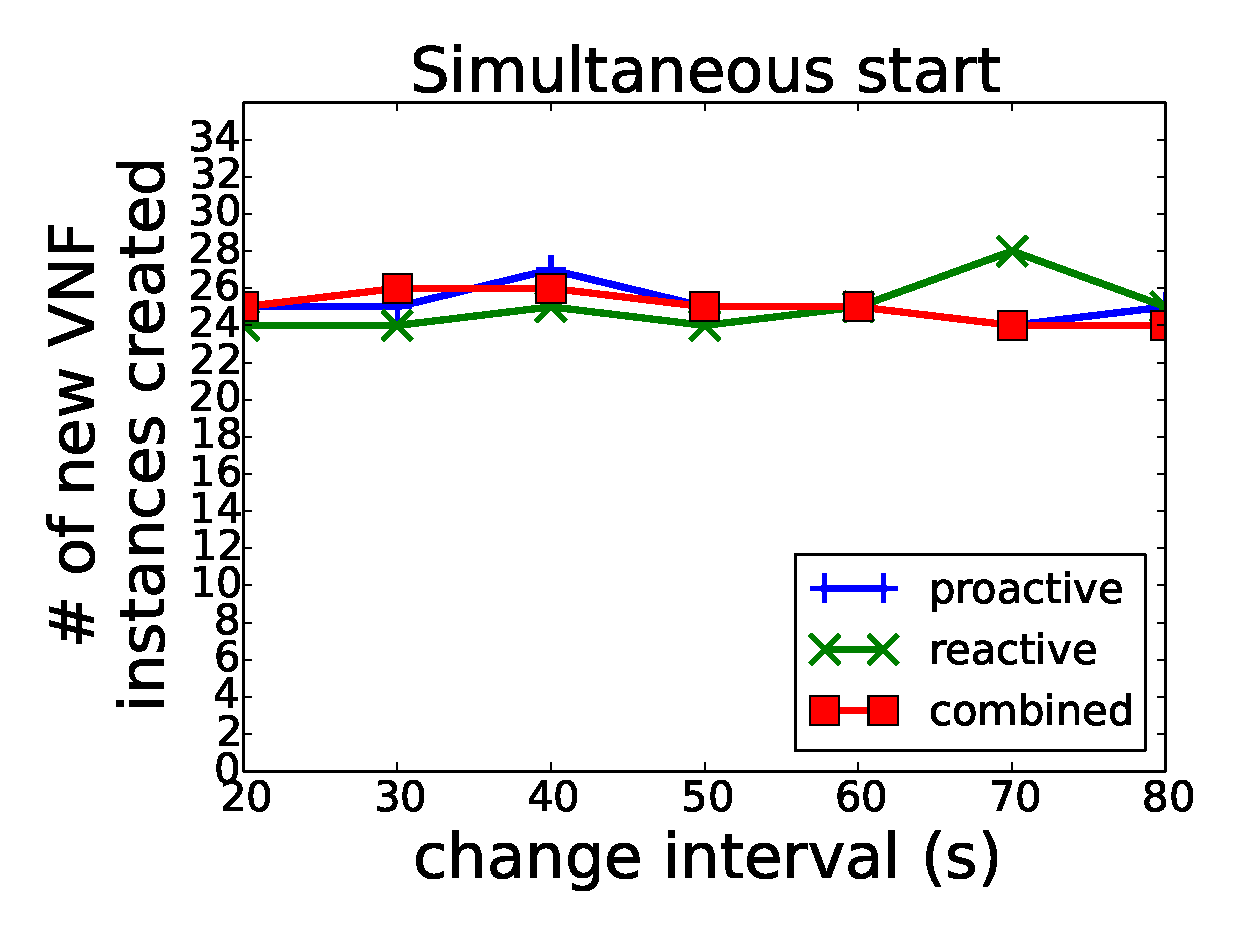
\includegraphics[width=\columnwidth]{chap-scalims/figure/nf-creation1.eps}
  \end{subfigure}
  \begin{subfigure}[t]{0.49\linewidth}
     \centering
     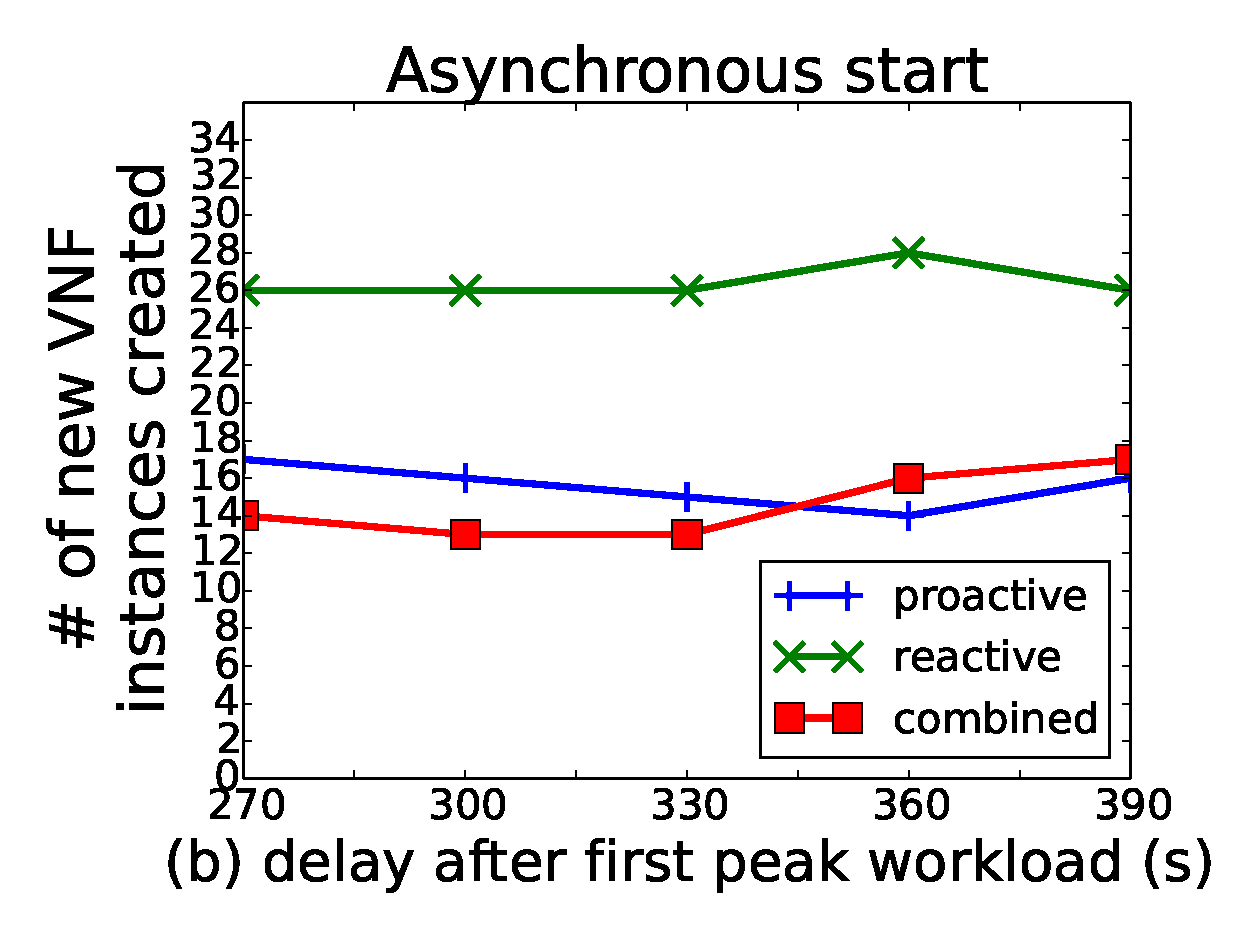
\includegraphics[width=\columnwidth]{chap-scalims/figure/nf-creation2.eps}
    \end{subfigure}
        \caption{Overall number of new VNF instances created: (a) simultaneous start; (b) asynchronous start.}
        \label{fig:nf-creation}
\end{figure}

\subsubsection{Simultaneous Start}

\begin{figure}[!h]
        \centering
        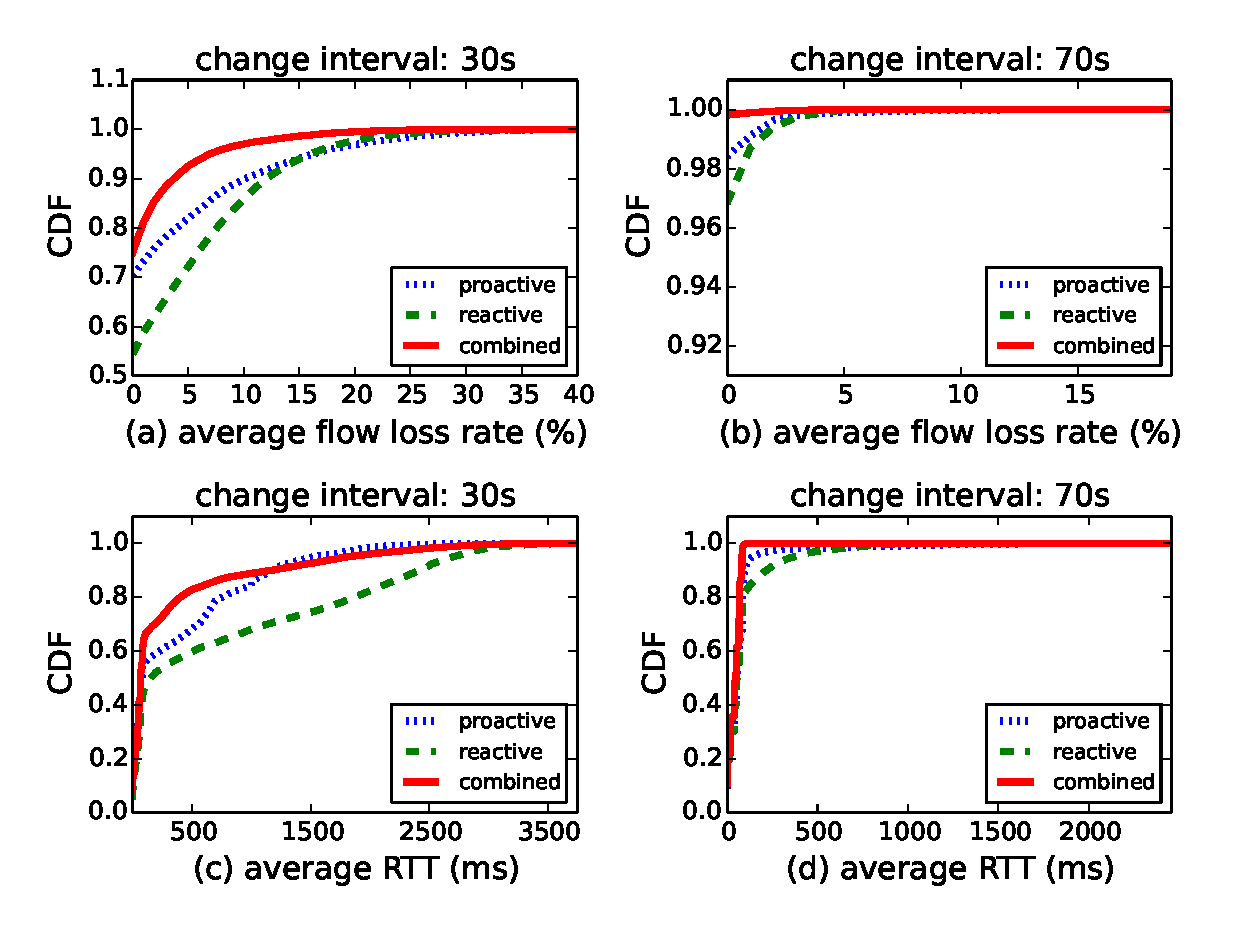
\includegraphics[width=\columnwidth]{chap-scalims/figure/syn-lossrate-rtt.eps}
        \caption{QoS of DP flows: simultaneous start.}
        \label{fig:syn-lossrate-rtt}
\end{figure}

\begin{figure}[!h]
  \begin{subfigure}[t]{0.49\linewidth}
   \centering
   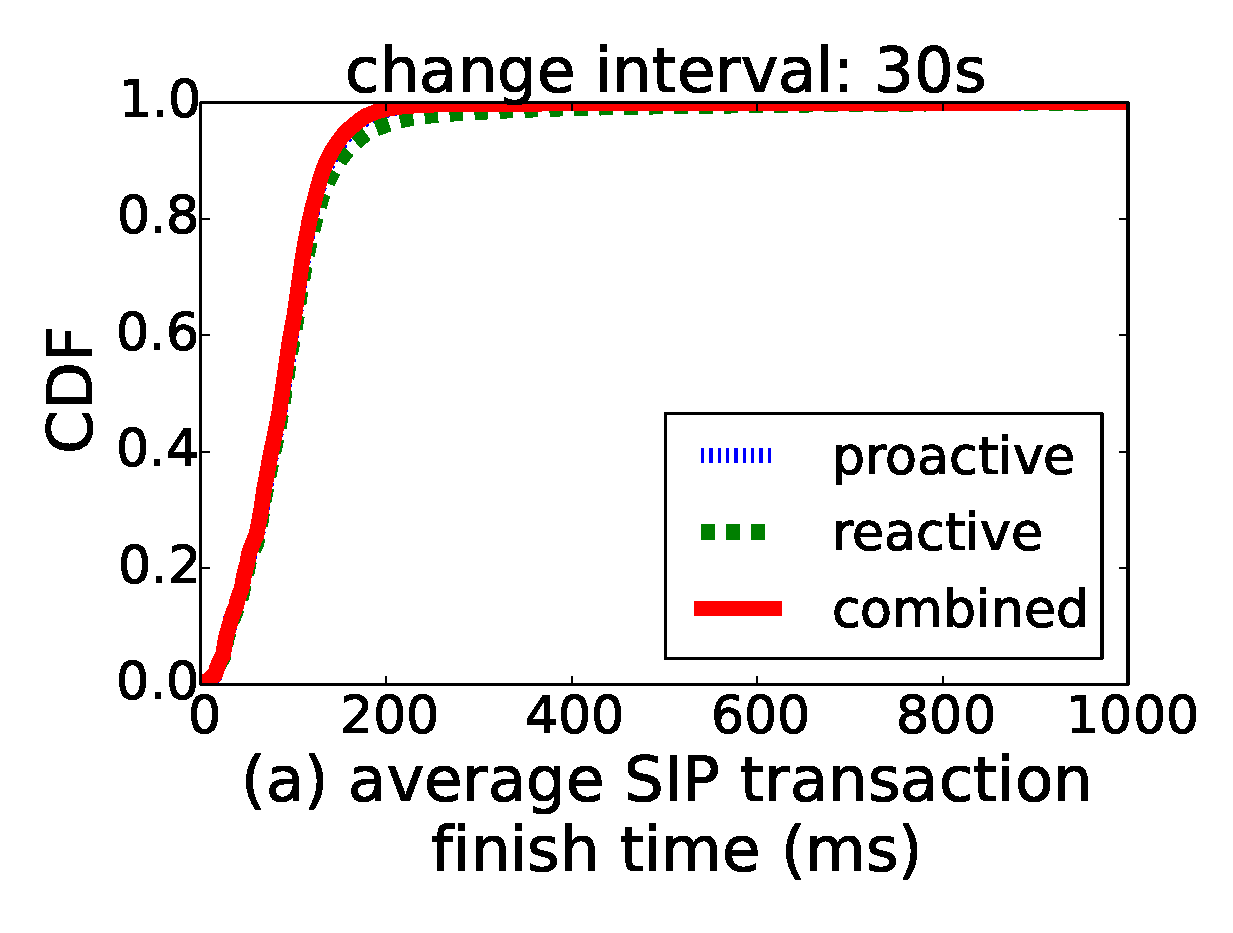
\includegraphics[width=\columnwidth]{chap-scalims/figure/syn-cp1.eps}
  \end{subfigure}
  \begin{subfigure}[t]{0.49\linewidth}
     \centering
     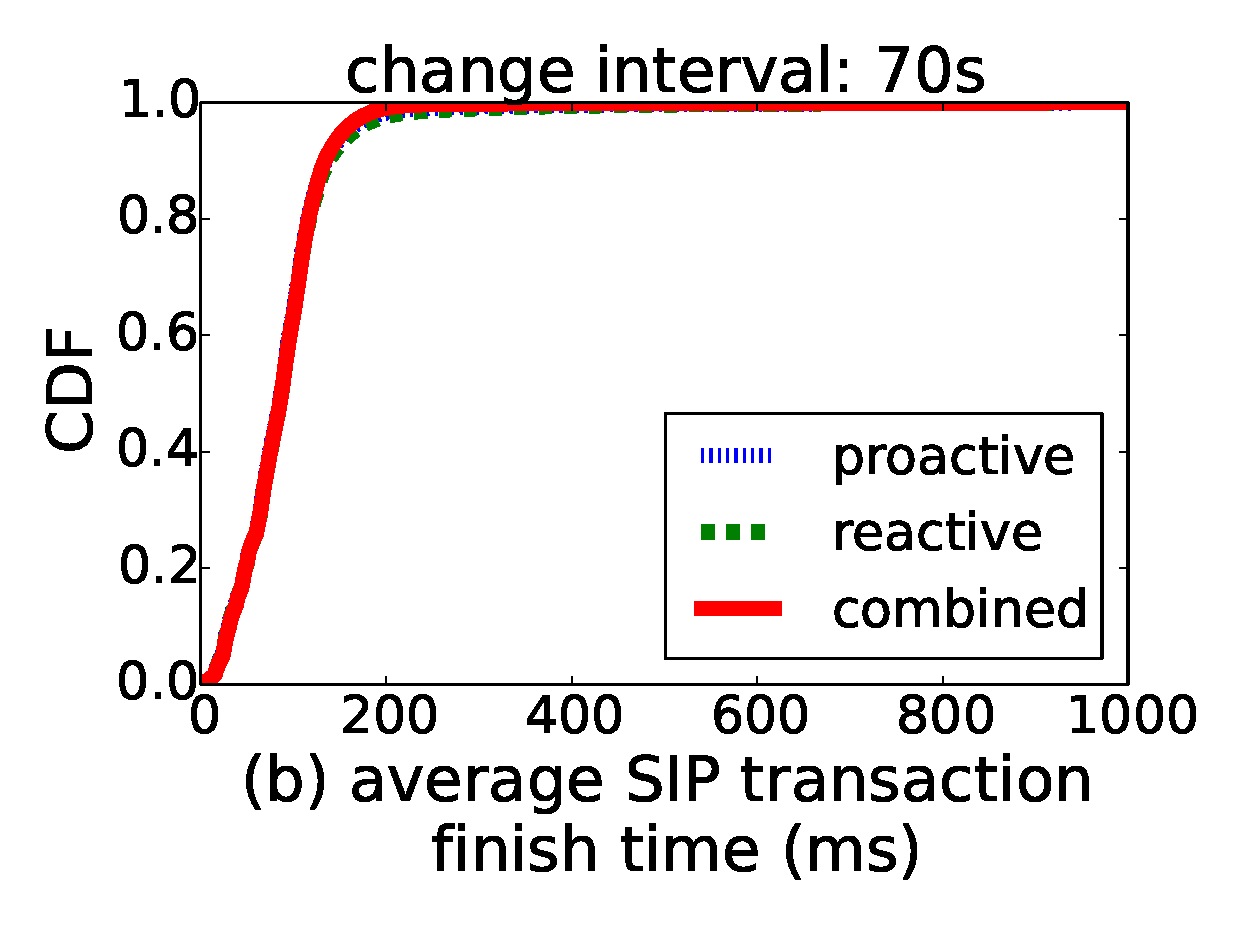
\includegraphics[width=\columnwidth]{chap-scalims/figure/syn-cp2.eps}
    \end{subfigure}
\caption{QoS of CP flows: simultaneous start.}
\label{fig:syn-cp}
\end{figure}

In this set of experiments, each traffic generator starts generating users simultaneously at the rate of $1~users/s$, which gradually increases to $15~users/s$ and then decreases to $6~users/s$. The rate change happens once every \textit{change interval}. The duration of change intervals is set to different values in different experiments.
 %All the traffic generators will start generating users simultaneously at the start of the experiment run,
In this way, the peak workload arrives at each datacenter almost concurrently. %The duration of a change interval is set to 20s, 30s, ... 80s respectively.

%(\chuan{Fig.~\ref{fig:nf-creation}(b): in y labels, instance should be instances'})

Fig.~\ref{fig:nf-creation}(a) shows that the total number of VNF instances provisioned (for both CP and DP service chains) does not differ much under the three schemes. Since the maximum workload on each datacenter arrives at around the same time, the proactive scaling algorithm has no opportunity to decrease the number of provisioned VNF instances by adjusting the service chain path, and therefore the numbers are similar.


Fig.~\ref{fig:syn-lossrate-rtt} plots CDFs of the number of DP flows at different average packet loss rates and average RTTs, and shows that the combined scaling strategy of {\em ScalIMS} out-performs the other two strategies in terms of DP traffic quality. %Due to limited space, we only present the DP traffic quality and CP traffic quality when updated interval is set to 20s and 80s in figure~\ref{fig:syn-lossrate-rtt} and figure~\ref{fig:syn-cp}.
%The reason can be explained as follows.
 Pure reactive scaling adds new instances only when overload occurs. During the boot-up time of new instances, traffic continues to arrive at the overloaded VNF instances, resulting in a high packet loss rate and then high RTT. Pure proactive scaling adjusts VNF instances once every scaling interval. During each scaling interval, increased workload may have overloaded the system. The best performance is achieved combining both proactive and reactive scaling.

Fig.~\ref{fig:syn-cp} shows that the average SIP transaction completion time is similar with the three schemes. This is because scaling of CP service chains is not triggered as often as DP service chains, since each instance of a CP VNF is able to handle a large number of SIP transactions. %Second, the overload threshold for CP VNF is set to a smaller value (70\% of the overload threshold), due to the fact that we observe constant CP VNF crash when CP VNF is on brink of overloading.

%We also Even though we can set a smaller threshold for overload detection to improve the performance of pure reactive scaling approach, but this will inevitably provision more NF instances and decrease resource utilization rate. In order to show this phenomena,

%I didn't managed to produce good result for this set of experiment on IBM cloud, has to delete it.
%To evalaute the impact of the overload threshold in reactive scaling, we conduct another set of experiments by running pure reactive scaling with thresholds set to 80\% of the default overload detection threshold. The results are shown as ``reactive 80\%" in Fig.~\ref{fig:syn-lossrate-rtt} and Fig.~\ref{fig:syn-cp}. We observe that even though decreasing the threshold improves the quality of the user traffic, the quality is still worse than the combined approach.% letting alone the additional created VNF instances during the experiment.

%Figure~\ref{fig:syn-cp} shows CP user traffic quality and performance of the 3 approaches are similar. First, CP scaling is not triggered very often as compared to DP, because CP VNF is able to handle a large amount of SIP transactions. Second, the overload threshold for CP VNF is set to a smaller value (70\% of the overload threshold), due to the fact that we observe constant CP VNF crash when CP VNF is on brink of overloading.

\subsubsection{Asynchronous Start}

\begin{figure}[!h]
  \begin{subfigure}[t]{0.49\linewidth}
   \centering
   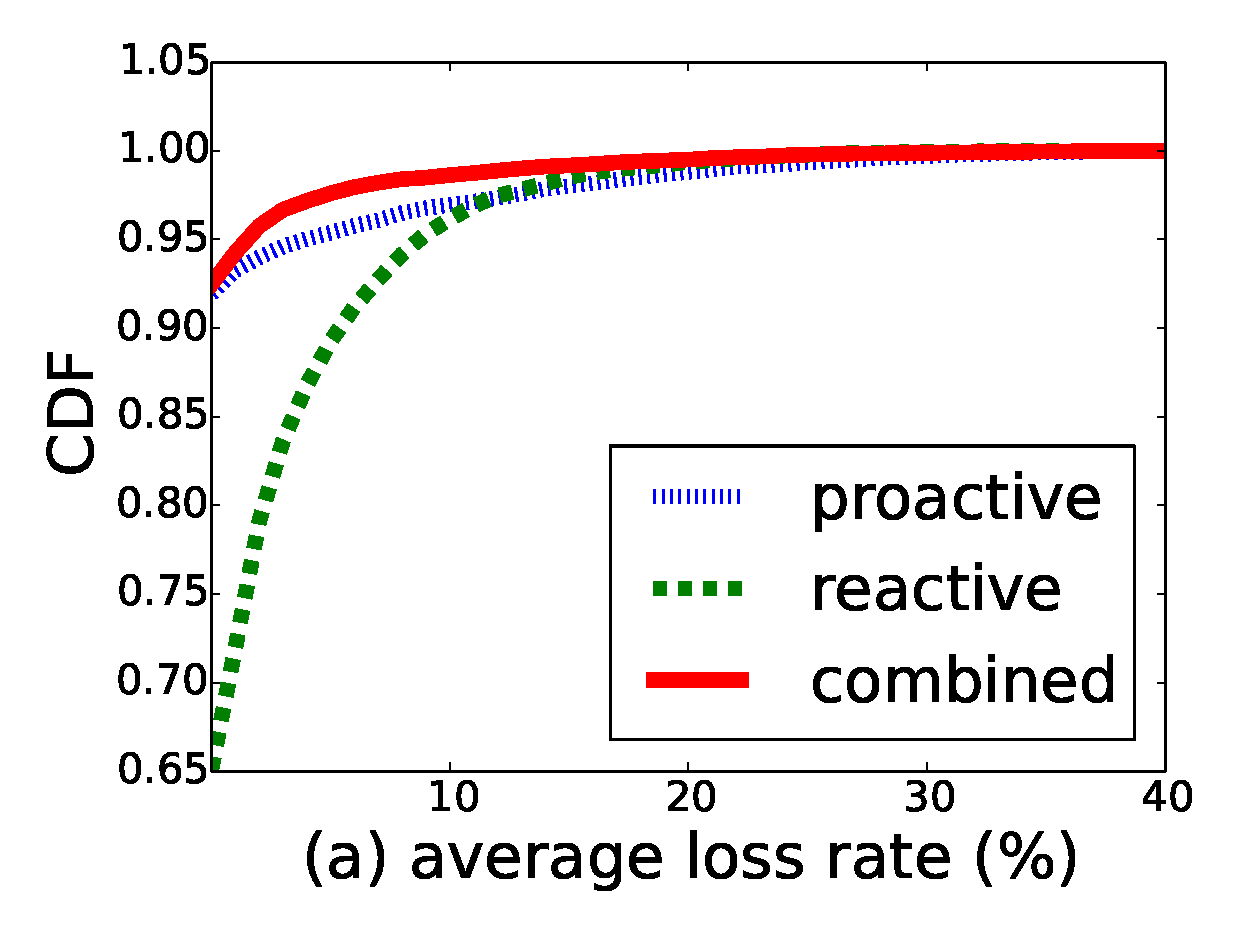
\includegraphics[width=\columnwidth]{chap-scalims/figure/nonsyn-rttloss1.eps}
  \end{subfigure}
  \begin{subfigure}[t]{0.49\linewidth}
     \centering
     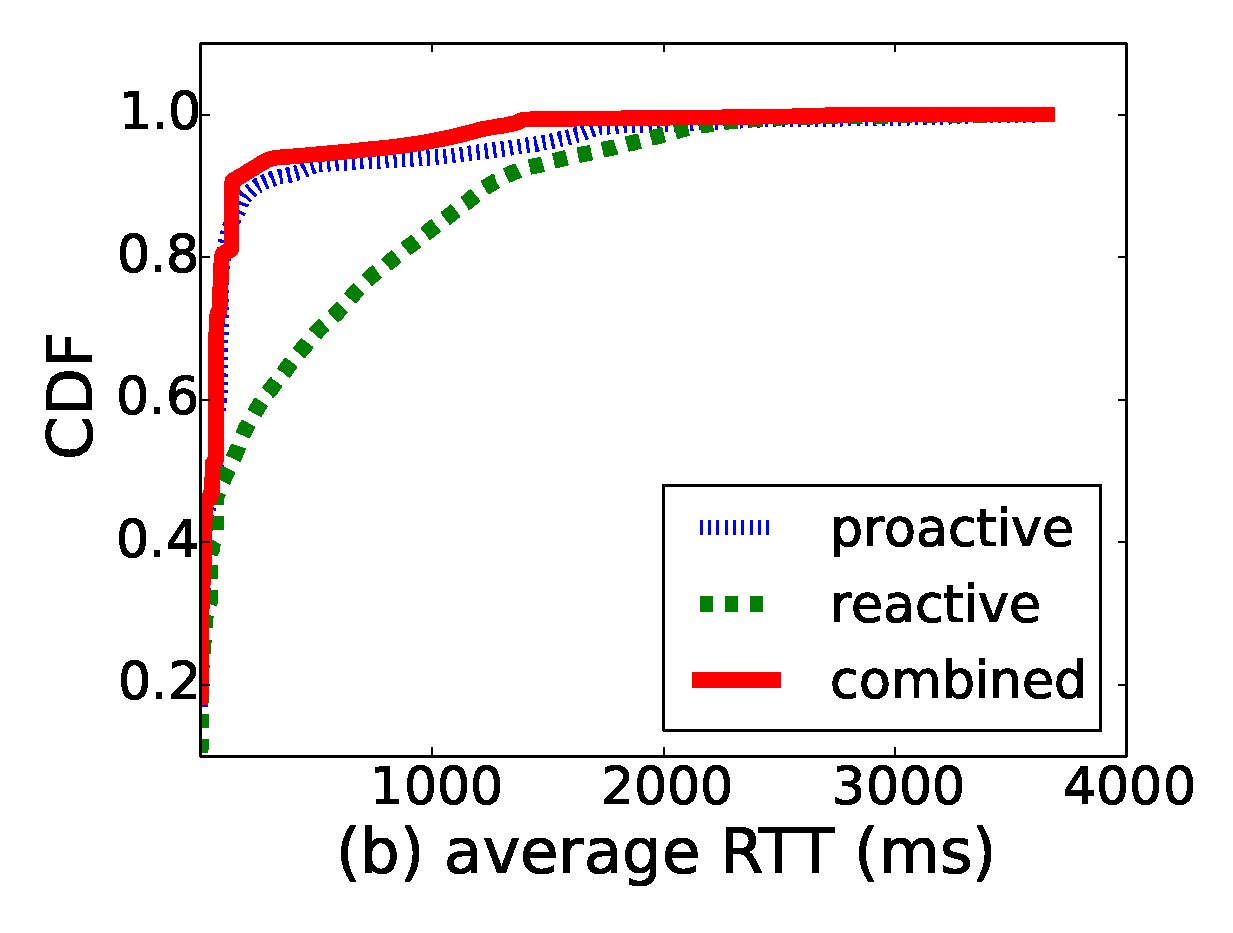
\includegraphics[width=\columnwidth]{chap-scalims/figure/nonsyn-rttloss2.eps}
    \end{subfigure}
\caption{QoS of DP flows: asynchronous start.}
\label{fig:nonsyn-rttloss}
\end{figure}

In this set of experiments, %traffic generators are not started at the same time.
the traffic generator in the Tokyo datacenter is started first, followed by the traffic generators in Hong Kong, in Houston and then in London. %The start time of the traffic generator in a subsequent datacenter is delayed for a configurable period of time after that of the previously started traffic generator.
 In this way, the peak workload in different datacenters does not occur at the same time. Each traffic generator increases its user generation rate from 5 $users/s$ to 15 $users/s$ and then reduces it to $5~users/s$, with a 30s change interval.

In Fig.~\ref{fig:nf-creation}(b), the start delay between traffic generators in Tokyo and in Hong Kong is set according to the values on the x axis, while start delays between traffic generators in Hong Kong and in Houston, and between traffic generators in Houston and in London, are set to 120s. We observe that the number of VNF instances created with the combined scaling approach is similar to proactive scaling approach, but always smaller than reactive scaling approach. Fig.~\ref{fig:nonsyn-rttloss} shows that the traffic quality is the best with the combined approach as well. The performance of CP SIP transaction completion time under asynchronous start is very similar to the results presented in Fig.~\ref{fig:syn-cp}. %Due to limited space, we show the DP traffic quality with 300s delay value in figure~\ref{fig:nonsyn-rttloss}. The combined approach out-performs reactive scaling by a large margin in terms of both flow loss rate and measured RTT.

%We can see that the number of provisioned NF instances in combined scaling approach is apparently smaller than that of purely reactive scaling approach. And even with smaller NF instance provision number, the combined scaling approach has a better data plane traffic quality than the reactive scaling approach.

\subsubsection{Explanation}

\begin{figure}[!h]
        \centering
        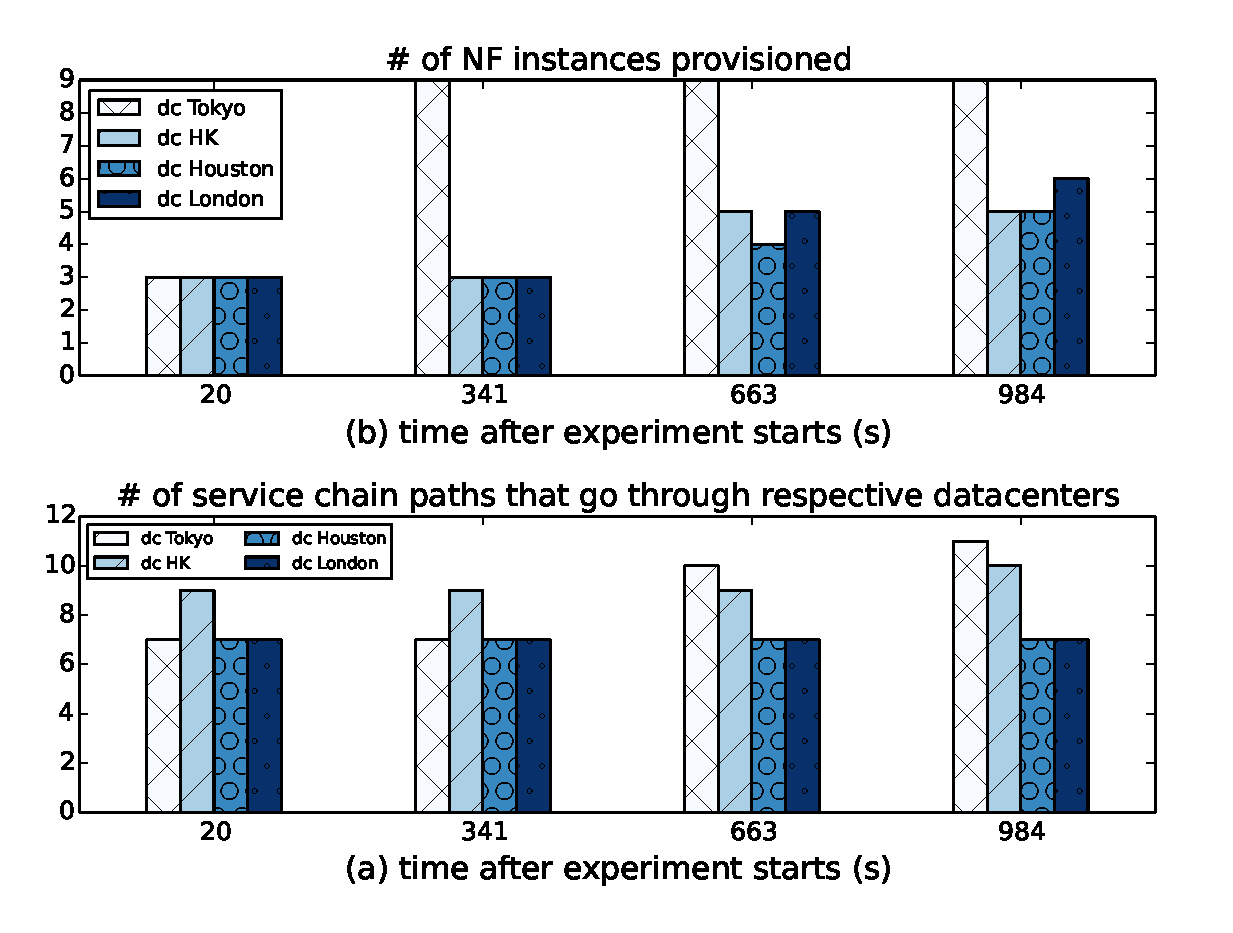
\includegraphics[width=1\columnwidth]{chap-scalims/figure/nonsyn-reason.eps}
        \caption{%Delayed start time is 300s
		%(a) Number of provisioned VNF instances in each datacenter versus time. (b) The number of service chain paths going through different datacenters.
		 Number of VNF instances in/service chain paths through each datacenter: asynchronous start.}
        \label{fig:nonsyn-scpath}
\end{figure}

Why can the combined scaling strategy perform well even when it creates a smaller number of VNF instances? The Tokyo datacenter sees the peak workload first, leading to the provisioning of many VNF instances in the datacenter, which later become redundant and will be buffered for 10 scaling intervals. When peak workload arrives at other datacenters, the global controller can re-use the buffered VNF instances by creating service chain paths traversing the Tokyo datacenter. %, increasing resource utilization efficiency. %We can see from the experiment results that as a side effect, traffic quality also gets improved. %The reason is illustrated in Fig.~\ref{fig:nonsyn-scpath}.
 These phenomena are exhibited in Fig.~\ref{fig:nonsyn-scpath}. %(a) shows the number of VNF instances created in each datacenter verses the time after the experiment starts. We can see that due to the early arrival of peak workload, many VNF instances are provisioned in Tokyo datacenter by 341s. After that time, the number of service chain paths that go through Tokyo datacenter increases from 7 to 11 (Fig.~\ref{fig:nonsyn-scpath}(b)) because the global controller schedules more DP traffic flows to re-use these existing VNF instances. Because these existing VNF instances are buffered and reused, DP traffic flows do not go through overloaded instances, improving the quality experienced by the DP flows.



%\subsection{Evaluation in an Emulation Cluster}

%We also evaluate the performance of \textit{ScalIMS} on our own computing cluster containing 8 IBM blade servers, each equipped with 16 cores, 80GB RAM, 500GB SATA disk, and connected to a Gigabyte Ethernet switch. We emulate a datacenter using a server. The inter-datacenter delay is emulated using Linux TC. By default, the 8 datacenters are separated into 4 groups (i.e. $g_0$ to $g_3$, where $g_i$ contains datacenter $i$ and $i+1$). Datacenters in same group are close to each other with an inter-datacenter delay of 5ms. Datacenters in different groups are farrer away from each other and their delays are set according to the corresponding inter-group delay shown in Table~\ref{table:stat}.

%\vspace{-3mm}
\begin{comment}
\subsection{Evaluation in Emulation Cluster}

%\subsubsection{Links with Large Delays}

We next investigate whether {\em ScalIMS} is able to effectively detect links with high delays and shift the traffic away from these links, using our own 8-server emulation cluster. We emulate a datacenter using one server, and vary inter-datacenter delays with Linux TC \cite{tc}. The 8 emulated datacenters are divided into 4 groups (i.e. $g_0$ to $g_3$, where $g_i$ contains datacenter $i$ and $i+1$). The delay between datacenters in the same group is set to 5ms, and the delay between datacenters in different groups is set according to Table~\ref{table:stat}.

In this set of experiments, traffic generators increase user production rate from 1 $user/s$ to 12 $users/s$ and then decrease the rate to 6 $users/s$, with a 50s change interval. The maximum allowed end-to-end flow delay is 50ms. At 350s after each experiment starts, we deliberately increase the delay between groups $1$ and $3$ to 65ms, and hence the global controller would avoid using links between groups $1$ and $3$.

\begin{figure}[!t]
  \begin{subfigure}[t]{0.49\linewidth}
   \centering
   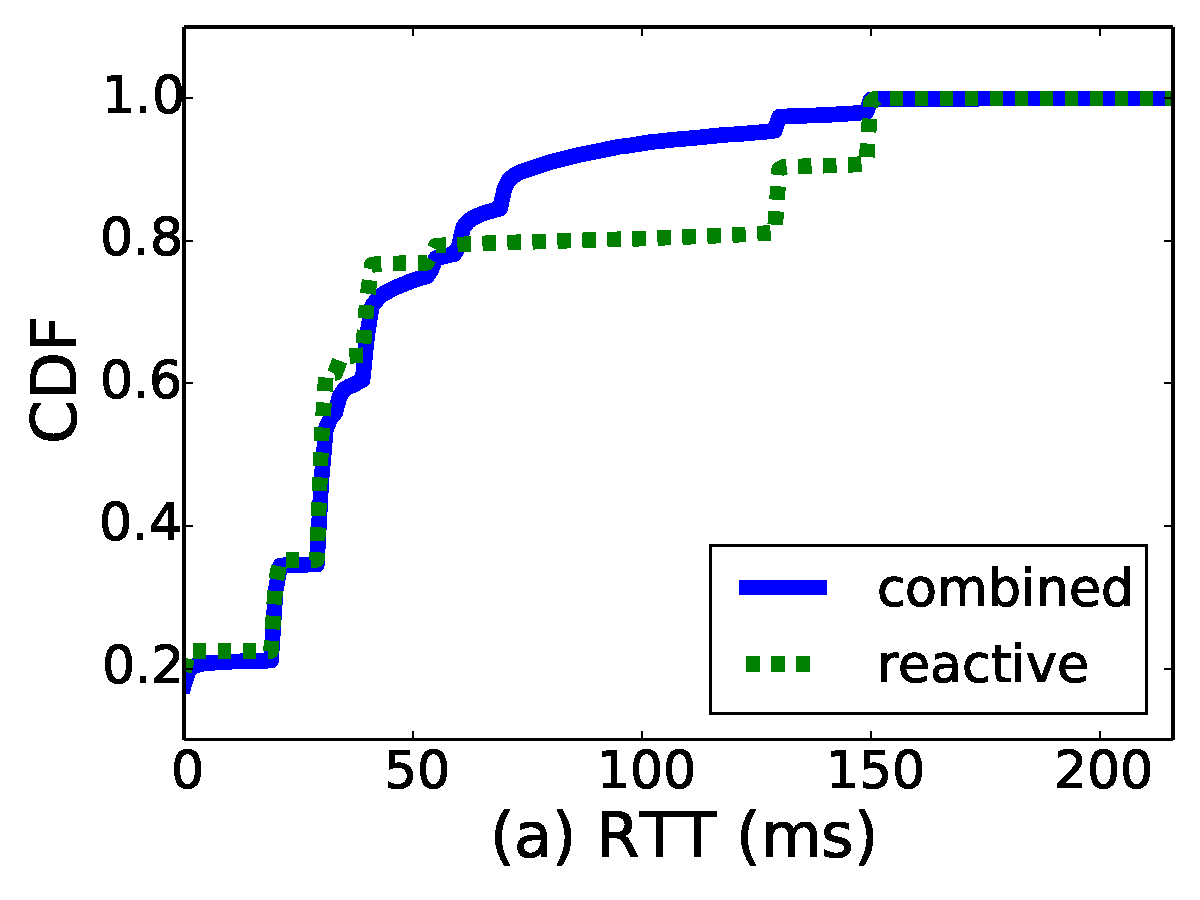
\includegraphics[width=\columnwidth]{chap-scalims/figure/delay1.pdf}
  \end{subfigure}
  \begin{subfigure}[t]{0.49\linewidth}
     \centering
     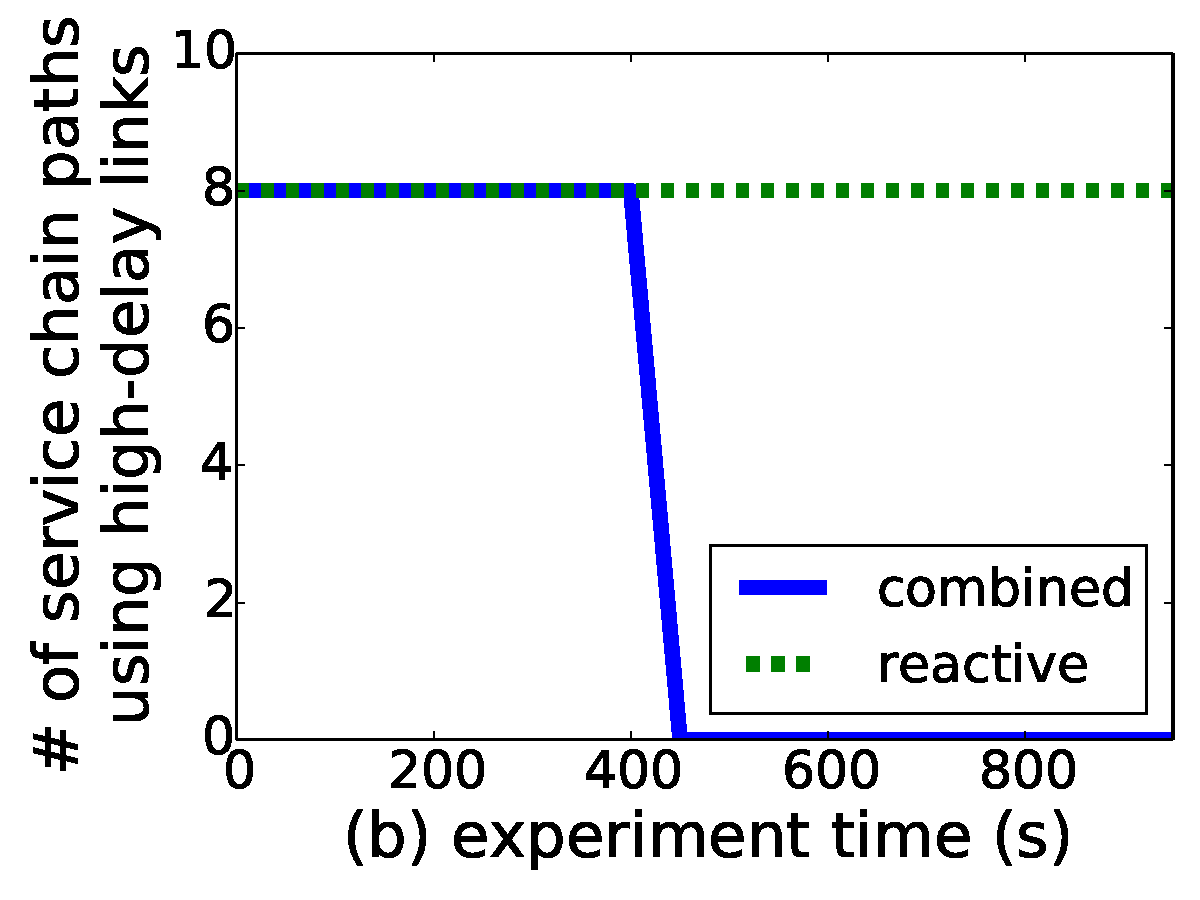
\includegraphics[width=\columnwidth]{chap-scalims/figure/delay2.pdf}
    \end{subfigure}
    \caption{Emulation results in case of links with large delays.}% (a) CDF of flow RTT. (b) Number of service chain paths that use the links between group 1 and group 3.}
    \label{fig:delayrun}
    \vspace{-5mm}
\end{figure}

%\begin{figure}[!t]
%        \centering
%        \includegraphics[width=1\columnwidth]{figure/delay.pdf}
%        \caption{Emulation results in case of links with large delays.}% (a) CDF of flow RTT. (b) Number of service chain paths that use the links between group 1 and group 3.}
%        \label{fig:delayrun}
%\end{figure}

Fig.~\ref{fig:delayrun} (a) shows that with {\em ScalIMS}, the number of flows whose average RTT is smaller than 100ms is 15\% more than that with the reactive scaling approach. Fig.~\ref{fig:delayrun}(b) illustrates that the global controller can effectively re-compute new service chain paths, avoiding the high-delay links. The result of the proactive scaling strategy is similar with the combined scaling strategy because they share the same path computation algorithm.
\end{comment}
% At about 400s, the number of service chain paths that use the high delay links drops from 8 to 0, boosting the quality of the DP media flow.


\begin{comment}
%\subsubsection{Scaling Interval Consistency}

We also evaluate the impact of our design on maintaining scaling interval consistency as discussed in Sec.~\ref{Inconsistency}, by comparing it with one where flows are not tagged with scaling intervals and local controllers always route flows using servcice chain paths in the current scaling interval. In this set of experiments, we generate 15 calls per second between datacenter 0 and 1 for 5 minutes. Enough VNF instances are pre-provisioned on 3 datacenters (datacenters $0-2$) to serve the traffic. The global controller alternates service chain paths from datacenter 0 to datacenter 1 and from datacenter 1 to datacenter 0 from (0, 0, 0, 1, 1) and (1, 1, 1, 0, 0) to (0, 2, 2, 2, 1) and (1, 2, 2, 2, 0) in each scaling interval. %The global controller is placed on datacenter 2, so that there is basically no delay between global controller and datacenter 2 local controller. On the other hand,
The delays between datacenters 0 and 2 and between datacenters 1 and 2 are both set to 400ms.
If a local controller finds out that it is not on a flow's service chain path, it applies a rule that drops all the packets of this flow. %The packet loss rates of all the generated flows are shown in Table~\ref{tab:con}.

%\textbf{First}, we run experiment with our distributed flow routing fully enabled. \textbf{Second}, we run experiment without scaling interval tagging, and force subsequent datacenters on service chain path to always use the service chain path under their current scaling interval.


We find that without scaling interval tagging, 18 out of 8722 flows ($0.2\%$) are completely not received by their receivers. On the contrary, all 8724 flows are received with 0\% loss rate when the scaling interval tagging is enabled. This is because when service chain paths from datacenter 0 to datacenter 1 and from datacenter 1 to datacenter 0 are switched from (0, 2, 2, 2, 1) and (1, 2, 2, 2, 0) to (0, 0, 0, 1, 1) and (1, 1, 1, 0, 0), datacenter 2 enters the next scaling interval earlier. There is a small time window when datacenter 2 starts using service chain path (0, 0, 0, 1, 1) and (1, 1, 1, 0, 0) while datacenter 0 and datacenter 1 are still in the previous scaling interval, using service chain path (0, 2, 2, 2, 1) and (1, 2, 2, 2, 0). Datacenters 0 and 1 continue sending flows to datacenter 2 during that time window, but datacenter 2 finds that it is not on the service chain path of this flow, thus dropping all the packets. We omit the related figures due to space constraint.
\end{comment}

\begin{comment}
\begin{table}[!t]
%\captionsetup{font=footnotesize}
\centering
\caption{Loss rate when scaling interval tagging is enabled/disabled}
\label{tab:con}
\resizebox{.9\columnwidth}{!}{
\begin{tabular}{|l|l|l|}
\hline
\begin{tabular}[c]{@{}l@{}}Loss rate \\ summary\end{tabular}                 & \begin{tabular}[c]{@{}l@{}}With scaling\\ interval tagging\end{tabular} & \begin{tabular}[c]{@{}l@{}}Without scaling\\ interval tagging\end{tabular} \\ \hline
\begin{tabular}[c]{@{}l@{}}\# of generated \\ flows\end{tabular}              & 8724                                                                    & 8722                                                                       \\ \hline
\begin{tabular}[c]{@{}l@{}}\# of flows with\\ 0\% packet loss\end{tabular}   & 8724                                                                    & 8704                                                                       \\ \hline
\begin{tabular}[c]{@{}l@{}}\# of flows with\\ 100\% packet loss\end{tabular} & 0                                                                       & 18                                                                         \\ \hline
\end{tabular}
}
\end{table}
\begin{comment}

\begin{comment}
\begin{table}[h]
\centering
\caption{Flow loss rate when scaling interval tagging is enabled/disabled}
\label{tab:con}
\resizebox{\columnwidth}{!}{
\begin{tabular}{|c|c|c|}
\hline
                                                                                      & \begin{tabular}[c]{@{}c@{}}With scaling\\ interval tagging\end{tabular} & \begin{tabular}[c]{@{}c@{}}Without scaling\\ interval tagging\end{tabular} \\ \hline
\begin{tabular}[c]{@{}c@{}}Number of flows with \\ 0\% packet loss rate\end{tabular}  & 8724                                                                    & 8704                                                                       \\ \hline
\begin{tabular}[c]{@{}c@{}}Number of flows with\\ 100\% packet loss rate\end{tabular} & 0                                                                       & 18                                                                         \\ \hline
\end{tabular}
}
\end{table}
\end{comment}
